\documentclass[12pt]{article}
\usepackage[spanish]{babel}

%%%%%%%%%%%%%%%%%%%%%%%%%%%%%%%%%%
%%%%%%%%%%%%%%%%%%%%%%%%%%%%%   %%
%%        Datos Trabajo     %%  %%
%%%%%%%%%%%%%%%%%%%%%%%%%%%%%%%%%%
\newcommand{\titulo}[0]{Actividad 2. Muestreo.}
\newcommand{\materia}[0]{Estadística Básica}
\newcommand{\grupo}[0]{BI-BEBA-2002-B2-013}
\newcommand{\unidad}[0]{Unidad 3}


%%%%%%%%%%%%%%%%%%%%%%%%%%%%%%%%%%
%%%%%%%%%%%%%%%%%%%%%%%%%%%%%%%%%%
\usepackage{amssymb}
\usepackage{enumerate}
\usepackage{geometry}
\usepackage{mathtools}
\usepackage{multicol}
\usepackage{soul}

\usepackage{graphicx}
	\graphicspath{ {assets/} }

\usepackage{hyperref}
	\hypersetup{
			pdftex,
		        pdfauthor={bench},
		        pdftitle={\titulo},
		        pdfsubject={\materia},
		        pdfkeywords={\grupo, \unidad, UnADM},
		        pdfproducer={Latex with hyperref, Ubuntu},
		        pdfcreator={pdflatex, or other tool},
			colorlinks=true,
				linkcolor=[rgb]{0,0,0.45},
				urlcolor=cyan,
				filecolor=green,
				citecolor=blue}

%%%%%%%%%%%%%%%%%%%%%%%%%%%%%%%%%%
%%%%%%%%%%%%%%%%%%%%%%%%%%%%%%%%%%

\title{
	
\includegraphics{../../../assets/logo-unadm} \\
	\ \\ Benjam\'in Rivera \\
	\bf{\titulo}\\\ \\}

\author{
	Universidad Abierta y a Distancia de México \\
	TSU en Biotecnolog\'ia \\
	\textit{Materia:} \materia \\
	\textit{Grupo:} \grupo \\
	\textit{Unidad:} \unidad \\
	\\
	\textit{Matricula:} ES202105994 }

\date{\textit{Fecha de entrega:} \today}


%%%%%%%%%%%%%%%%%%%%%%%%%%%%%
%%        Documento         %%
%%%%%%%%%%%%%%%%%%%%%%%%%%%%%%%
\begin{document}
\maketitle\newpage

\subsection*{Intruducci\'on}

	\par En esta unidad se analizan técnicas de muestreo, y el porque son utiles en el estudio y analizis de datos recolectados. Para reafirmar esto me agrado la frase que se menciona en el libro
	
	\begin{quote}
		\it Si los datos muestrales no se reúnen en forma adecuada resultarían tan inútiles que ningún grado de tortura esadística podría salvarlos. \footnote{\cite[p 6]{basica}}
	\end{quote}
	
	\noindent de donde me parece que queda bastante clara la importancia del muestreo.
	
\section*{Muestreo}
	\begin{figure}[h]
		\centering
		\includegraphics[scale=0.08]{Muestra_estadística.png}
		\caption{Mapa conceptual de muestreo. Mejor resolución en los anexos.}
		\label{mapa conceptual}
	\end{figure}
		
\section*{Ejercicio}

	\par En un lote de $25000$ cajas de medicina se desea verificar que la proporción de los ingredientes activos sea el adecuado. Se debe determinar el tamaño de la muestra para un nivel de confianza de $95\%$ con un error del $5\%$ si la variabilidad es $p = q = 0.5$
	\ \\\ \\\noindent \textbf{Solución}
	\par Dado que no tenemos mucha informaci\'on pasaremos a usar el muestreo aleatorio simple.
	\par Primero debemos definir la poblaci\'on y el parametro de estudio. Esto ya esta definido en la descripci\'on del problema, de manra que la poblaci\'on es el conjunto de cajas y el parametro de interes es el porcentaje de diabilidad de los ingredientes.
	\par Luego definiremos que cada caja tenga un \textit{ID} \'unico para poder identificarlas, que seran numeros entre 1 y 25000.
	\par Despues de esto podemos notar que el tama\~no de la poblaci\'on en este ejercicio es $N=25000$. Tambi\'en debemos notar que el nivel de confianza de $95\%$, consideramos un error del $5\%$ y una variabilidad de $p = 1-q = 0.5$
	\par Con estos datos podemos pasar a definir el tama\~no ideal de la muestra, lo que se puede calcular con la siguiente f\'ormula.
	$$ n = \frac{Z^2 p q N}{NE^2 + Z^2 p q} = \frac{1.95^2 * 0.5 * (1 - 0.5) * 25000}{25000*0.05^2 + 1.95^2*0.5*0.5} = 374.55 \sim 376 $$
	
	\par Por \'ultimo es necesario seleccionar a los candidatos. Este paso se muestra en las capturas de pantalla de excel.
	
	\begin{figure}[htp]
\centering
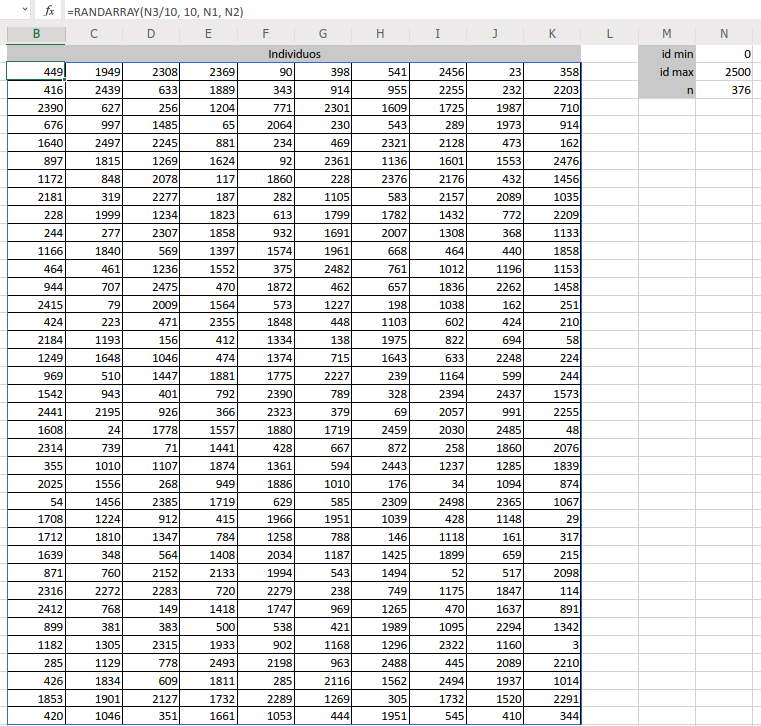
\includegraphics[scale=0.6]{muestras.png}
\caption{Muestra generada aleaoriamente en excel}
\label{muestras}
\end{figure}




%%%%%%%%%%%%%%%%%%%%%%%%%%%%%%%%
%%         Bibliografia        %%
%%%%%%%%%%%%%%%%%%%%%%%%%%%%%%%%%%
\newpage
\begin{thebibliography}{X}
	\bibitem{basica} Universidad Abierta y a Distancia de México. (s/f). \textit{Unidad 3. Representación numérica y gráfica de datos}. UnADM.
 
\end{thebibliography}

\end{document}